\documentclass[11pt,a4paper]{scrartcl}
\usepackage{graphicx}                    
\usepackage{mathtools}                   
\usepackage{amsmath,amssymb}            
\usepackage{multicol}                    
\usepackage{hyperref}    
\usepackage{xurl}                        
\usepackage[utf8]{inputenc}             
\usepackage[T1]{fontenc}                
\usepackage{enumitem}
\usepackage{float}
\usepackage[inkscapelatex=false]{svg}
\usepackage[
  style=authoryear,
  backend=biber,
  maxcitenames=2,   
  maxbibnames=99   
]{biblatex}

\DeclareCiteCommand{\textcite}
  {\boolfalse{cbx:parens}}
  {\usebibmacro{citeindex}%
   \printtext[bibhyperref]{\printnames{labelname}}%
   \setunit{\addspace}%
   \printtext[bibhyperref]{%
     \printtext[parens]{\usebibmacro{cite:labeldate+extradate}}}}
  {\multicitedelim}
  {\usebibmacro{textcite:postnote}}

\addbibresource{references.bib}
\DeclareFieldFormat{pages}{#1}
\newbibmacro*{pages}{\printfield{pages}}


\DefineBibliographyExtras{english}{%
  \protected\def\mkbibetal{\emph{et\addabbrvspace al\adddot}}%
}
\renewcommand*{\nameyeardelim}{\space}


\DeclareNameAlias{author}{family-given}
\DeclareFieldFormat[article]{title}{#1}
\renewbibmacro*{date}{%
  \printtext[parens]{\printfield{year}}%
}
\DeclareFieldFormat{pages}{#1}
\renewbibmacro*{journal+issuetitle}{%
  \printfield[journaltitle]{journaltitle}%
  \setunit*{\addcomma\space}%
  \printfield{volume}%
  \iffieldundef{number}{}{%
    \printfield[parens]{number}%
  }%
  \setunit{\addcolon}%
  \printfield{pages}%
}
\renewbibmacro*{pages}{}
\DeclareBibliographyDriver{article}{%
  \printnames{author}%
  \setunit{\labelnamepunct}\newblock
  \usebibmacro{date}%
  \newunit\newblock
  \printfield{title}%
  \newunit\newblock
  \usebibmacro{journal+issuetitle}%
  \finentry
}



\title{\textbf{Exercise 3 – using \LaTeX}}
\author{John Gamboa, Shaiban Alshaibani, Damla Nur Imirzalioglu}
\date{August 8, 2025}


\begin{document}

\maketitle
This course, and the course that preceded it, has probably been a lot of work. In the first course, you learned how to use \texttt{git}, learned about Python classes, and used
PsychoPy to generate your own study. In the second course (that is, this one), you
learned a bit about code-switching and switching costs, learned how to use \texttt{plotnine},
and pre-processed some real data using pandas. With this last exercise, you will finish
the course by producing (or, indeed, \textit{reproducing}) a document with \LaTeX.

\section{LaTeX basics: In case you didn’t come to the classes}
A lot of the materials in the two courses introduced in detail the main things you needed
to know about each of the “methods” you were learning. Hence, you had a .pdf explaining
in detail how to use \texttt{plotnine}, and another one explaining a lot of the details on how to
use \texttt{pandas}. The case of LaTeX is different. I preferred to go for a “normal” classroom
exposition of what I deemed important.

This was for a good reason. As I mentioned in the class, the internet is teeming with
webpages explaining how to do just about \textit{anything} with LaTeX (including programming,
indeed!), and it would be a huge waste of time and resources to write \textit{yet another} tutorial
about it. Instead, I decided to just link you to some materials I felt were a nice start.
They won’t have exactly the same content you saw in the class, but, hopefully, with
the knowledge you acquire by consuming them, you won’t have too much difficulty in
figuring out how to do any additional things that are not present there. Here they are:


\begin{itemize}
    \item The Wikibooks has \href{https://en.wikibooks.org/wiki/LaTeX}{a great Wikibook on LaTeX} that you are encouraged to take a look at;
    \item A great tutorial on how to start using LaTeX is \href{https://ctan.kako-dev.de/info/lshort/english/lshort.pdf}{The Not So Short Introduction to LaTeX} that will give you many details on the language;
    \item If you prefer videos, this \href{https://www.youtube.com/watch?v=ydOTMQC7np0}{Code Camp tutorial} is great;
    \item If nothing else works, the great Google (or your other search engine of choice) is your friend =)
\end{itemize}


In previous versions of this file, I would have recommended you to install LaTeX.
Unfortunately, depending on the operating system you use (surprisingly, Windows users
may have the upper hand in this case), LaTeX may be way too large to install only to
write a single assignment. In this case, you may want to use the \href{https://sharelatex.rz.rptu.de}{Overleaf server hosted by the University}.
 Overleaf is a webpage (\href{https://www.overleaf.com}{\texttt{www.overleaf.com}}) in
which you can create an account and make your own LaTeX projects. You’ll have to sign up to use it, so, the drawback of doing that is that they’ll have your data (which is more valuable than you may think). 

Alternatively, Overleaf is also a software that you can install on a computer. This
computer, then, works as a server, and other computers (the clients) can access the
computer to run their own LaTeX projects. In this case, it is the main computer (the
server) that will have your data. This is what our university has: you can log in to the
Overleaf server using your RHRK account.

If you do decide to use Overleaf, make sure to transfer the files from Overleaf to your
git repository when your submission is ready, so that I can see your code (more about
this in the next section).

\section{What is the assignment?}
Instead of following the precedent of the previous exercises—where I walked you through
the entire assignment using the data from \textcite{gade2021}, and then asked you to use
the knowledge you acquired to work on the data from \textcite{gosselin2024}—this
exercise is relatively straightforward:

\begin{quote}
Your job is to recreate this very document verbatim using LaTeX.
\end{quote}


That is, you need to produce a LaTeX code (a .tex\footnote{\texttt{exercise03\_replica.tex}} file,  
a .bib\footnote{\texttt{references.bib}} file, and a .svg\footnote{\texttt{Figure\_2\_GadeEtAl.svg}} file)  
that will generate a .pdf\footnote{\texttt{exercise03\_replica.pdf}} that looks identical to this one. Each of these files must be submitted (see Section~\ref{2.2}). To work on your code, you can use whichever platform you prefer (e.g., you can install LaTeX on your computer, or use Overleaf).


The \textbf{only} differences between this document and the one that will be generated by
your code should be the third author (which you should replace with your actual name)
and the date of your document. Your submission should be otherwise identical to this
.pdf file when compiled.

\newpage
\subsection{Some information you will need}
You may find it useful to know that the \verb|\documentclass{}| used to create this file is
called \texttt{scrartcl} (which works just like the class article, but with some additional
functionality parameters), using 11-point font on A4 paper (you will need to find out
how to set this). Additionally, the following packages were imported in the preamble:

\begin{multicols}{2}
\begin{enumerate}[label=\roman*.]
    \item \texttt{hyperref}
    \item \texttt{mathtools}
    \item \texttt{multicol}
    \item \texttt{natbib}
    \item \texttt{svg}
    \item \texttt{xurl}
\end{enumerate}
\end{multicols}

\subsection{What exactly do I need to submit?}
\label{2.2}
In your repository, make a folder called Exercise 3, where you will put the LaTeX code
corresponding to your submission. You should include the output of that code (i.e. a
.pdf file) and, importantly, the following three files required to compile that output:

\begin{itemize}
    \item A file called \texttt{exercise03\_replica.tex}, containing the LaTeX code you used to
reproduce your “copy” of this exercise;
    \item A file called \texttt{references.bib}, containing the bibliographic information necessary
to correctly generate this .pdf file (see \hyperref[References]{References});
    \item  A file called \texttt{Figure\_2\_GadeEtAl.svg}, which can be created by referring to \textit{Python
Code Snippet} 8 in Exercise 1.
\end{itemize}

I require these because, regardless of the platform you use to create the LaTeX code,
I will run the following command lines to test your submission (indeed, you can also use
them to check if your code works):

\begin{quote}
\begin{verbatim}
$ pdflatex exercise03_replica.tex

$ bibtex exercise03_replica.aux

$ pdflatex exercise03_replica.tex

$ pdflatex exercise03_replica.tex
\end{verbatim}
\end{quote}

\newpage
\section[Some things we’ve seen from Gade et al. (2021)]{Some things we’ve seen from \textcite{gade2021}}

In the last two exercises, we processed and made graphs of the data provided by \textcite{gade2021}. This data was a summary of the L1 and L2 switching-costs found in several
papers. It looked more or less like \autoref{table1}.


\vspace{1em}
\begin{table}[H]
\caption{Sample of data \texttt{GadeEtAl simplified.csv}, made using
\texttt{tablesgenerator.com}}
\label{table1}
\resizebox{\columnwidth}{!}{%
\begin{tabular}{|l|c|c|c|c|c|}
\hline
\multicolumn{1}{|c|}{\textbf{Study}} & \textbf{NumberOfStudy} & \textbf{Paradigm} & \textbf{L1sc} & \textbf{L2sc} & \textbf{Dominance} \\ \hline
Blanco-Elorrieta \& Pykkaenen, 2017  & 1                      & cued              & 116           & 90            & 77                 \\
Blanco-Elorrieta \& Pykkaenen, 2017  & 1                      & cued              & 33            & -2            & 24.5               \\
Blanco-Elorrieta \& Pykkaenen, 2017  & 1                      & voluntary         & 23            & 15            & -60                \\
Bonfienie et al., 2019               & 2                      & cued              & 45            & 64            & 34.5               \\
Bonfienie et al., 2019               & 2                      & cued              & 39            & 50            & 32.5               \\
\multicolumn{1}{|c|}{...}            & ...                    & ...               & ...           & ...           & ...                \\
Zhu \& Sowman 2020                   & 73                     & cued              & 5             & 33            & 100                \\
Zhu \& Sowman 2020                   & 73                     & cued              & 18            & 23            & 7.5                \\
Zhu \& Sowman 2020                   & 73                     & cued              & -15           & 4             & 22.5               \\
Zhu \& Sowman 2020                   & 73                     & cued              & 22            & 16            & 7                  \\
Zhu \& Sowman 2020                   & 73                     & cued              & 13            & 17            & 20                 \\ \hline
\end{tabular}%
}
\end{table}



The paper looked at the costs experienced by speakers when moving from their L1 to
their L2 (their \textit{L2 switch cost}, \texttt{L2sc}), or from their L2 to their L1 (their \textit{L1 switch cost}, \texttt{L1sc}). 
The data the authors analyzed (recall that it was a meta-analysis) had two types
of trials (“Repeat” and “Switch” trials), along with reaction times associated with each
of these conditions. The switch costs were calculated by subtracting the “Repeat” trial
reaction times from the “Switch” trial reaction times.


Even though the authors used the terms “L1” and “L2” in their scripts (the code
they wrote to analyze the data), their data actually did not use the terms “L1” or “L2”,
but rather “dominant” and “non-dominant” language. Thus, their switch costs were
calculated as:\footnote{LaTeX is especially known for having a very powerful “sub-language”, able to produce any sort of nice math notation. The Wikibook on LaTeX has two very useful chapters on it that you are more than encouraged to take a look at in order to recreate the formulas above: \href{https://en.wikibooks.org/wiki/LaTeX/Mathematics}{here} and 
\href{https://en.wikibooks.org/wiki/LaTeX/Advanced_Mathematics}{here}.

Note also that you can use the character $\sim$ (tilde) to insert additional spaces between the terms of an equation}

\begin{center}
\begin{tabular}{l}
\texttt{data['L1sc'] = data['RT dominant switch']} \\
\texttt{\phantom{data['L1sc'] = } - data['RT dominant repeat']} \\[0.5em]
\texttt{data['L2sc'] = data['RTnon dominant switch']} \\
\texttt{\phantom{data['L2sc'] = } - data['RTnon dominant repeat']}
\end{tabular}
\end{center}

\newpage
Along with these costs, they also calculated a measure that they referred to as “Dominance”. Dominance was calculated as:

\[
\begin{aligned}
\texttt{data['Dominance']} &={}\\
&\hspace{-6em}\dfrac{\begin{pmatrix}
\texttt{data['RT dominant switch']}\\
+\ \texttt{data['RT dominant repeat']}
\end{pmatrix}}{2}
- \dfrac{\begin{pmatrix}
\texttt{data['RTnon dominant switch']}\\
+\ \texttt{data['RTnon dominant repeat']}
\end{pmatrix}}{2}
\end{aligned}
\]




In plain words, the \texttt{Dominance} column (you can see some of its values in \autoref{table1}) was calculated by taking the average of the “Switch” and “Repeat” reaction times for the dominant language, and subtracting, from it, the average of the “Switch” and “Repeat” reaction times for the non-dominant language.


This Dominance measure, calculated above, was then used to produce Figure 2 of \textcite{gade2021} (here, referred to as \autoref{figure1}):

\begin{figure}[h] 
    \centering
    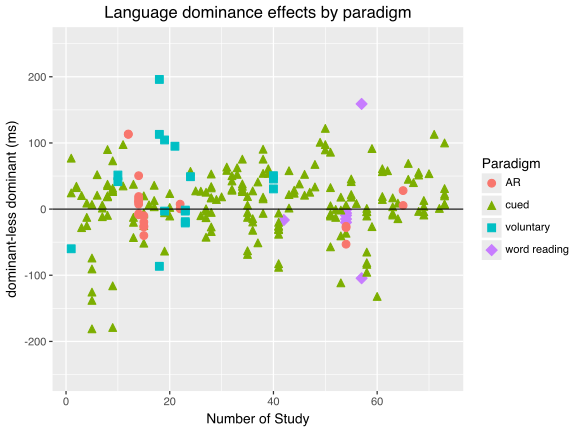
\includegraphics[width=0.7\textwidth]{Figure_2_GadeEtAl.png} 
    \caption{Recreation of Figure 2 from Gade et al.}
    \label{figure1}
    \label{fig:gade}
\end{figure}

%\begin{figure}[t!]
%\centerline{\includesvg[width=0.75\columnwidth]{Figure_2_GadeEtAl.svg}}
%\caption{Figure 1: Recreation of Figure 2 from Gade et al.}
%\label{fig: example}
%\end{figure}

\newpage
\section{“Completion Criteria”}
Of course, you already knew all of this that we discussed above. This whole story is
there just so you have \textit{something} to “reproduce”.


In order to have concluded this exercise, all you need to do is to produce a LaTeX
file whose output looks identical to it. Given that this exercise has a clear completion
criteria (either you successfully reproduced the file or not), the list below does not \textit{really}
contain actual “Completion Criteria”, but rather a number of things you should attend
to while producing your replica. I will at least check the following:

\begin{itemize}
    \item Whether your figures, tables, formulas, captions, headers and footnotes are \textbf{identical} to the Exercise definition.
    \item Whether your references are correctly formatted (and correctly used), both in the text and in the References section.
    \item Whether your hyperlinks work.
    \item Whether you correctly formatted the text as \textbf{bold}, \textit{italic}, \texttt{code}, etc.
\end{itemize}

\section{Final remarks}
Once you are done reproducing this file, and assuming that you have already finished
the other exercises (Exercises 1 and 2), you will have successfully concluded this course.
After the submission deadline, I will take a look at the files you submitted and, unless I
find any major problems, I will give you the credits in QIS.


As mentioned earlier, this course was a lot of work. The knowledge you acquired
through these exercises goes well beyond the “methods” – you not only learned tools
that will likely be required in your research career, but you also practiced a lot of
programming with Python, exploring new language functionalities that had not yet
been introduced in the first semester. Given how heavy the course was, I would like to
thank you for having persisted until the end. It was a great pleasure to have taught you,
and it is my most sincere hope that this course will be useful for your future.


Good luck with your next steps in either building experiments or analyzing data,
regardless of whether it is with or without Python =]

\printbibliography[title={References}]
\label{References}





\end{document}

